\let\negmedspace\undefined
\let\negthickspace\undefined
\documentclass[journal]{IEEEtran}
\usepackage[a5paper, margin=10mm, onecolumn]{geometry}
%\usepackage{lmodern} % Ensure lmodern is loaded for pdflatex
\usepackage{tfrupee} % Include tfrupee package

\setlength{\headheight}{1cm} % Set the height of the header box
\setlength{\headsep}{0mm}     % Set the distance between the header box and the top of the text

\usepackage{gvv-book}
\usepackage{gvv}
\usepackage{cite}
\usepackage{amsmath,amssymb,amsfonts,amsthm}
\usepackage{algorithmic}
\usepackage{graphicx}
\usepackage{textcomp}
\usepackage{xcolor}
\usepackage{txfonts}
\usepackage{listings}
\usepackage{enumitem}
\usepackage{mathtools}
\usepackage{gensymb}
\usepackage{comment}
\usepackage[breaklinks=true]{hyperref}
\usepackage{tkz-euclide} 
\usepackage{listings}
% \usepackage{gvv}                                        
\def\inputGnumericTable{}                                 
\usepackage[latin1]{inputenc}                                
\usepackage{color}                                            
\usepackage{array}                                            
\usepackage{longtable}                                       
\usepackage{calc}                                             
\usepackage{multirow}                                         
\usepackage{hhline}                                           
\usepackage{ifthen}                                           
\usepackage{lscape}
\usepackage{circuitikz}
\tikzstyle{block} = [rectangle, draw, fill=blue!20, 
    text width=4em, text centered, rounded corners, minimum height=3em]
\tikzstyle{sum} = [draw, fill=blue!10, circle, minimum size=1cm, node distance=1.5cm]
\tikzstyle{input} = [coordinate]
\tikzstyle{output} = [coordinate]


\begin{document}

\bibliographystyle{IEEEtran}
\vspace{3cm}

\title{4.8.35}
\author{AI25BTECH11039-Harichandana Varanasi}
 \maketitle
% \newpage
% \bigskip
{\let\newpage\relax\maketitle}

\renewcommand{\thefigure}{\theenumi}
\renewcommand{\thetable}{\theenumi}
\setlength{\intextsep}{10pt} % Space between text and floats


\numberwithin{equation}{enumi}
\numberwithin{figure}{enumi}
\renewcommand{\thetable}{\theenumi}



\date{}

\begin{document}
\maketitle



\textbf{Question.} Find the coordinates of the foot of the perpendicular drawn from the point $\myvec{0\\1\\2}$ on the $x\text{-axis}$
.

\textbf{Solution.}
Let the $x\text{-axis}$
 be represented as the intersection of the two planes
\[
\vec{e}_2^{\,T}\vec{x}=0,\quad \vec{e}_3^{\,T}\vec{x}=0,
\]
where
\[
\vec{e}_1=\myvec{1\\0\\0},\ \vec{e}_2=\myvec{0\\1\\0},\ \vec{e}_3=\myvec{0\\0\\1}.
\]
The direction vector of the $x\text{-axis}$
 is $\vec{m}=\vec{e}_1$ and the given point is
\[
\vec{P}=\myvec{0\\1\\2}.
\]

By the foot\text{-}of\text{-}perpendicular relation,

\begin{align}
\myvec{\vec{m}&\vec{e}_2&\vec{e}_3}^{\!T}\vec{Q}
=\myvec{\vec{m}^{T}\vec{P}\\[2pt]0\\[2pt]0}.
\tag{1}
\end{align}
Substituting $\vec{m}=\vec{e}_1$ and $\vec{P}=\myvec{0\\1\\2}$,
\begin{align}
\myvec{1&0&0\\[2pt]0&1&0\\[2pt]0&0&1}\vec{Q}
=\myvec{0\\[2pt]0\\[2pt]0}
\ \Longrightarrow\ 
\vec{Q}=\myvec{0\\0\\0}.
\tag{2}
\end{align}

Thus, the foot of the perpendicular from $\myvec{0\\1\\2}$ to the $x\text{-axis}$
 is
\[
\boxed{\myvec{0\\0\\0}}.
\]



\begin{figure}[H]
    \centering
    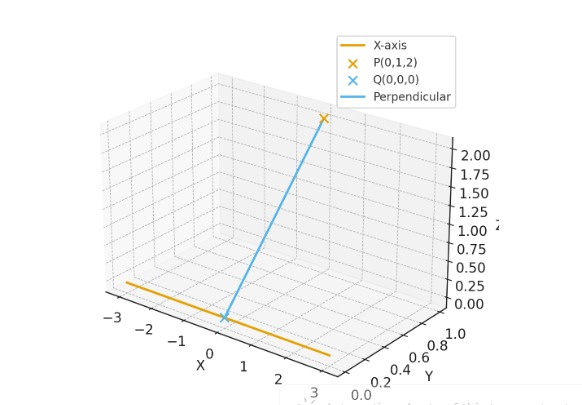
\includegraphics[width=0.75\linewidth]{figs/matgeo-4.8.35.jpeg}
    \caption{Perpendicular from $\vec{P}=\myvec{0\\1\\2}$ to thethe $x\text{-axis}$
 with foot $\vec{Q}=\myvec{0\\0\\0}$.}
    \label{fig:4.8.35-3d}
\end{figure}



 

\end{document}
